% Session 4 -- lowest-Landau-level orbitals as nested rings, and the uniform
% droplet they add up to at nu=1 and at nu=1/3.
% Placement: sec. "Angular momentum, enclosed flux, and the uniform electron gas".
% Rendered by figures/blender/s04f05_droplet.py, labels in figures/overlays/s04f05_droplet.tex.
\begin{aqmfigure}{fig:s04:droplet}{Angular momentum fixes the radius. (a) The lowest-Landau-level
orbitals (4.10), $|\psi_m|^2\propto r^{2m}e^{-r^2/2\ell_B^2}$, for $m=0,2,4,6,8$, each renormalized
here to the same peak height and cut open over half a turn. They are nested rings, and when $m$
increases the ring moves outward, to $r_m=\sqrt{2m}\,\ell_B$, and encloses more flux. (b) When we
add every orbital from $m=0$ to $m=N-1$ we therefore fill a disc, and the rings overlap in such a
way that the total density is flat inside the disc and falls off sharply at the edge. The filled
lowest Landau level is a uniform electron droplet without structure, with one electron per flux
quantum. The Laughlin state (4.12) at $\nu=1/3$ is the second profile. The same $N$ electrons now
use orbitals up to $m=3(N-1)$, so the radius of the droplet grows by $\sqrt{3}$ and the density
becomes a third, while the droplet stays as uniform as before. The Laughlin construction is built to
keep this uniformity, and the profiles of (b) are schematic.}
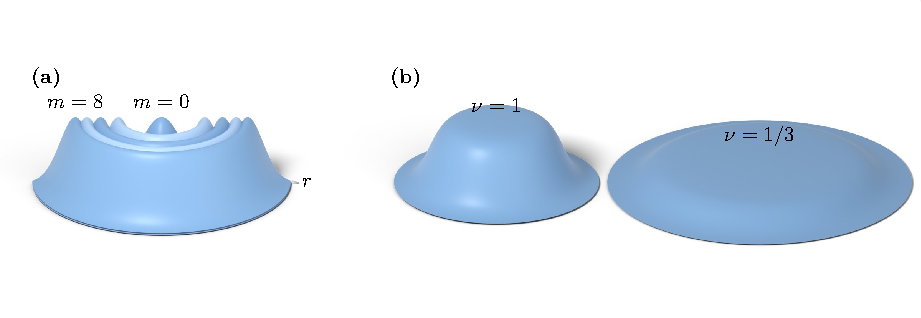
\includegraphics{figures/pdf/s04f05_droplet.pdf}
\end{aqmfigure}
